%Para slide em "Wide-Screen" usar:
\documentclass[aspectratio=43]{beamer} 

%Para slide "quadrado" usar:
%\documentclass{beamer} 

\usepackage{tikz}

%Elaborado por Mateus Moro Lumertz

\author{mateuslumertz}
\definecolor{cor1}{RGB}{0,100,166}
\definecolor{cor2}{RGB}{100,195,213}
\definecolor{cor5}{RGB}{150,203,226}
\definecolor{cor3}{RGB}{30,130,186}
\definecolor{cor4}{RGB}{40,185,218}
\definecolor{preto}{RGB}{0,0,0}
\definecolor{branco}{RGB}{255,255,255}
% Configuração das Cores
\setbeamercolor{paleta1}{fg=cor1,bg=white}
\setbeamercolor{paleta2}{fg=cor1,bg=white}
\setbeamercolor{estrutura}{fg=cor1,bg=white}
\setbeamercolor{titulo_rodape}{fg=black,bg=white}
\setbeamercolor{data_rodape}{fg=gray,bg=white}
\setbeamercolor{frametitle}{fg=branco,bg=cor1}

% Modelo do rodapé
\defbeamertemplate*{footline}{mytheme}{%
  \leavevmode%
  \hbox{\begin{beamercolorbox}[wd=.5\paperwidth,ht=2.5ex,dp=1.125ex,leftskip=.3cm,rightskip=.3cm]{titulo_rodape}%
    \makebox[2em][l]{{\usebeamerfont{titulo_rodape}\textcolor{cor1}{\insertframenumber}}}%
    {\usebeamercolor{titulo_rodape}\insertshorttitle}
  \end{beamercolorbox}%
  \begin{beamercolorbox}[wd=.2\paperwidth,ht=2.5ex,dp=1.125ex,leftskip=.3cm,rightskip=.3cm]{data_rodape}%
    \usebeamerfont{data_rodape}\insertshortdate%
  \end{beamercolorbox}%
  \begin{beamercolorbox}[wd=.3\paperwidth,ht=2.5ex,dp=1.125ex,leftskip=.3cm,rightskip=.3cm,right]{titulo_rodape}%
    
\includegraphics[width=.2\paperwidth,height=7ex,keepaspectratio]{imagens/logo.png}\hspace*{2em}%
  \end{beamercolorbox}}%
  \vskip0pt%
}

% Slide de Título
\defbeamertemplate*{title page}{mytheme}[1][]
{%
  \begin{tikzpicture}[remember picture,overlay]
    \filldraw[cor1]
    (current page.north west) --
    ([yshift=-12cm]current page.north west) --
    ([xshift=-4cm,yshift=-12cm]current page.north east) {[rounded corners=15pt]--
    ([xshift=-4cm,yshift=3cm]current page.south east)} --
    ([yshift=3cm]current page.south west) --
    (current page.south west) --
    (current page.south east) --
    (current page.north east) -- cycle
    ;
  \filldraw[branco]
    (current page.north west) --
    ([yshift=-2.15cm]current page.north west) --
    ([xshift=-3cm,yshift=-2.15cm]current page.north east) {[rounded corners=15pt]--
    ([xshift=-3cm,yshift=3cm]current page.south east)} --
    ([yshift=3cm]current page.south west) --
    (current page.south west) --
    (current page.south east) --
    (current page.north east) -- cycle
    ;
    \filldraw[cor2]
    ([xshift=-0.25cm,yshift=3cm]current page.south east)--
    ([xshift=-2.75cm,yshift=3cm]current page.south east)--
    ([xshift=-2.75cm,yshift=3.85cm]current page.south east)--
    ([xshift=-0.25cm,yshift=3.85cm]current page.south east)-- cycle
    ;
    \filldraw[cor3]
    ([xshift=-0.25cm,yshift=4cm]current page.south east)--
    ([xshift=-2.75cm,yshift=4cm]current page.south east)--
    ([xshift=-2.75cm,yshift=4.85cm]current page.south east)--
    ([xshift=-0.25cm,yshift=4.85cm]current page.south east)-- cycle
    ;
    \filldraw[cor4]
    ([xshift=-0.25cm,yshift=5cm]current page.south east)--
    ([xshift=-2.75cm,yshift=5cm]current page.south east)--
    ([xshift=-2.75cm,yshift=5.85cm]current page.south east)--
    ([xshift=-0.25cm,yshift=5.85cm]current page.south east)-- cycle
    ;
    \filldraw[cor5]
    ([xshift=-0.25cm,yshift=6cm]current page.south east)--
    ([xshift=-2.75cm,yshift=6cm]current page.south east)--
    ([xshift=-2.75cm,yshift=6.85cm]current page.south east)--
    ([xshift=-0.25cm,yshift=6.85cm]current page.south east)-- cycle
    ;
  \node[text=branco,anchor=south west,font=\sffamily\LARGE,text width=.68\paperwidth] 
  at ([xshift=10pt,yshift=-0.5cm]current page.west)
  (title)
  {\raggedright\inserttitle};  
  
  \node[text=cor1,anchor=south west,font=\sffamily\small,text width=.75\paperwidth] 
  at ([xshift=10pt,yshift=3.6cm]current page.west)
  (title)
  {\raggedright Université Côte d'Azur};  
  
  \node[anchor=east]
  at ([xshift=-0.15cm,yshift=-1cm]current page.north east)
  {
\includegraphics[width=2.5cm]{imagens/logo.png}};
  
  \node[text=preto,font=\large\sffamily,anchor=south west]
  at ([xshift=30pt,yshift=0.5cm]current page.south west)
  (date)
  {\insertdate};
  \node[text=preto,font=\large\sffamily,anchor=south west]
  at ([yshift=5pt]date.north west)
  (author)
  {\insertauthor};
  \end{tikzpicture}%
}

% remove navigation symbols
\setbeamertemplate{navigation symbols}{}

% definition of the itemize templates
\setbeamertemplate{itemize item}[circle]
\setbeamercolor{itemize item}{fg=cor3,bg=white}
\setbeamercolor{itemize subitem}{fg=cor4,bg=white}
\setbeamercolor{itemize subsubitem}{fg=cor2,bg=white}

%%%%%%%%%%%%%%%%%%%%%%%%%%%%%%%%%%%%%%%%%%%%%%%%%%%%%%%%%%%%%%%%%%%%
%%%%%%%%%%%%%%%%%%%%%%%%%%%%%%%%%%%%%%%%%%%%%%%%%%%%%%%%%%%%%%%%%%%%
%%%%%%%%%%%%%%%%%%%%%%%%%%%%%%%%%%%%%%%%%%%%%%%%%%%%%%%%%%%%%%%%%%%%
%%%%%%%%%%%%%%%%%%%%%%%%%%%%%%%%%%%%%%%%%%%%%%%%%%%%%%%%%%%%%%%%%%%%
%%%%%%%%%%%%%%%%%%%%%%%%%%%%%%%%%%%%%%%%%%%%%%%%%%%%%%%%%%%%%%%%%%%%

\title[Efficient Greedy Learning of GMM]{Efficient Greedy Learning of Gaussian Mixture Models (2003)
\newline \small{J.J. Verbeek, N. Vlassis B. Kröse -- \textit{U. of Amsterdam}}}
\author{Quentin Le Roux - MSc Data Science \& AI}
\date{\today}

\begin{document}

\begin{frame}[plain]
\maketitle
\end{frame}

%Slide 
\begin{frame}
    \frametitle{Overview of the paper}
    \framesubtitle{Aims}
    This paper draws from the literature on Gaussian Mixture Models (abb. GMM) to \textbf{propose a new method to improve on the standard Expectation-Maximization algorithm} (abb. EM).\linebreak
    \begin{small}\begin{itemize}
      \item It aims at \textbf{solving GMM's current sensitivity to/dependence on initialization};
      \item \textbf{locating a global maximum}, which EM cannot achieve;
      \item with a similar time complexity to be an acceptable and comparable algorithm to EM.
    \end{itemize}\end{small}
\end{frame}

%Slide 
\begin{frame}
    \frametitle{Overview of the paper}
    \framesubtitle{Gaussian-Mixture Models reminder}
    A $k$-component GMM is a linear combination of $k$ Gaussian distributions in $d$-dimensions:

    $$f_k(x)=\underset{i=1}{\overset{k}{\sum}}\pi_i.\phi(x|\mu_i,\Theta_i)$$
    $$\forall i \in \{1,...,k\}, \quad \pi_i\ge0, \quad\underset{i=1}{\overset{k}{\sum}}\pi_i=1, \quad \mu_i \in \mathbb{R}^d,\quad\Theta_i\in\mathbb{R}^{d\times d}$$
    $$\phi(x|\mu_i,\Theta_i) = \frac{1}{\sqrt{(2.\pi)^d.det(\Theta_i)}}.exp(-\frac{(x-\mu_i)^T.\Theta^{-1}.(x-\mu_i)}{2})$$\newline
    with $\pi$ the mixing weights and $\phi$ the components of the mixture, and with $\mu$ the mean and $\Theta$ the covariance matrix of a Gaussian density.
\end{frame}

%Slide 
\begin{frame}
    \frametitle{Overview of the paper}
    \framesubtitle{Expectation-Maximization reminder}
    EM is a standard algorithm for estimating the GMM parameters. It proceeds as such:
    \begin{small}\begin{enumerate}
      \item \textbf{Initialization}: Initial parameters (mean, covariance values) are initialized with an algorithm (e.g. K-Means) or randomly
      \item \textbf{E}(xpectation)\textbf{-step}: Computes a value $P(j|x_i)=\frac{\pi_j.\phi(x_i|\mu_j,\Theta_j)}{f_k(x_i)}$
      \item \textbf{M}(aximization)\textbf{-step}: Estimates new parameters sets $\{\mu\}$, $\{\Theta\}$, and $\{\pi\}$ for all components $j\in \{1,...,\}$:\linebreak
          $\pi_j=\underset{i=1}{\overset{n}{\sum}}\frac{P(j|x_i)}{n};\,\, \mu_j=\underset{i=1}{\overset{n}{\sum}}\frac{P(j|x_i).x_i}{n.\pi_j};\,\, \Theta_j=\frac{\underset{i=1}{\overset{n}{\sum}}P(j|x_i).(x_i-\mu_j)(x_i-\mu_j)^T}{n.\pi_j}$
      \item \textbf{Repeat steps 2 and 3 until a predefined convergence condition is met}  (e.g. The attribute \textit{tol} for sklearn's GMM. EM stops when the lower bound average gain is below it).
    \end{enumerate}\end{small}
\end{frame}

%Slide 
\begin{frame}
    \frametitle{Overview of the paper}
    \framesubtitle{Arising problems}
    \begin{itemize}
      \item Strong dependence on initialization\newline
      \item No possibility to take a peek into the model as it trains\newline
      \item no guarantee to have a global optimum
    \end{itemize}
\end{frame}

%Slide 
\begin{frame}
    \frametitle{Overview of the paper}
    \framesubtitle{The paper's innovation: a new [efficient, greedy] learning method - 1}
    If EM-based GMM is an \textbf{all-at-once} training algorithm, the papers proposes a \textbf{greedy} algorithm ( it is a process that makes the optimal choice at each step).
    \begin{small}\begin{itemize}
      \item Instead of starting with a configuration with all components and improving it, the mixture is \textbf{grown} component-wise, i.e., by adding each component one after the other
      \item \textbf{Intuition}: 
      \begin{itemize}
        \item It splits the optimization into easy-to-solve blocks
        \item Theoretical result (Kullback-Leibler divergence) implies the procedure can quickly approximate any density
        \item The mixture obtained at each step can inform better model building
      \end{itemize}
    \end{itemize}\end{small}
\end{frame}

\begin{frame}
    \frametitle{Overview of the paper}
    \framesubtitle{The paper's innovation: a new [efficient, greedy] learning method - 2}
    The greedy learning of Gaussian mixtures proceeds as such:
    \begin{small}\begin{enumerate}
      \item Compute the optimal (yielding maximal log-likelihood\footnote{\begin{scriptsize}$\mathcal{L}(X_n, f_k) = \underset{i=1}{\overset{n}{\sum}}log\,f_k(x_i)$ log-likelihood of the dataset $X_n$ under the k-component mixture $f_k$.\end{scriptsize}}) of the 1-component mixture $f_1$ ($k=1$)
      \item \textbf{Find the optimal new component} $\phi(x|\mu^\ast, \Theta^\ast)$ and corresponding mixing weight $\pi^\ast$ with $f_k$ fixed:
      $$\{\mu^\ast, \Theta^\ast, \pi^\ast\} = arg\, \underset{\{\mu, \Theta, \pi\}}{max}\underset{i=1}{\overset{n}{\sum}}log[(1-\alpha).f_k(x_i)+\alpha\phi(x_i, \mu, \Theta)]$$
      \item Set $f_{k+1}(x)=(1-\alpha^\ast)f_k(x)+\alpha^\ast\phi(x,\mu^\ast,\Theta^\ast)$ and $k += 1$
      \item \textit{Optional}: \textbf{Update $f_k$ using EM until convergence}
      \item \textbf{Repeat steps 2, 3 and 4 until a convergence condition is met}
    \end{enumerate}\end{small}
\end{frame}

%Slide 
\begin{frame}
    \frametitle{Overview of the paper}
    \framesubtitle{Results}
    The results presented in the paper:
    \begin{itemize}
      \item Used randomly generated datasets drawn from Gaussian mixtures, and sets of texture image data
      \item Shows that the efficient greedy method \textbf{outperforms the standard EM}
      \item while running at a $O(nk^2)$ time complexity, a factor of $k$ slower than standard EM, i.e. \textbf{$\frac{k}{2}$ times slower on average}\newline
    \end{itemize}
    The main benefit of this new method is:
    \begin{itemize}
      \item \textbf{independency from initialization}
      \item \textbf{facilitating a better model selection} (because a sequence of mixtures is created)
    \end{itemize}
\end{frame}

%Slide 
\begin{frame}
    \frametitle{References}
    \framesubtitle{_}
    \begin{itemize}
      \item Dempster, Laird, Rubin (1977) Maximum likelihood from incomplete data via the EM algorithm. \textit{Journal of the Royal Statistical Society}, 39(1):1-38
      \item Kullback, Leibler (1951) On Information and Sufficiency. Ann. Math. Statist. 22, no. 1, 79--86
    \end{itemize}
\end{frame}

%Slide
\begin{frame}
\frametitle{Note 1}
\framesubtitle{Efficient Search for New Components}
    When trying to find the component for the greedy algorithm presented in step 2 page 7, the paper mentions two methods:
    \begin{small}\begin{enumerate}
      \item \textbf{old method}: every data point generates a candidate (the point is the mean of a corresponding candidate with the same covariance matrix $\sigma^2.\mathbb{I}$). It yields $n$ candidates in a $O(n^2)$ time complexity, which is unacceptable in most application
      \item \textbf{new method}: the paper proposes to generates few good candidates
    \end{enumerate}\end{small}
\end{frame}

%Slide
\begin{frame}
\frametitle{Note 2}
\framesubtitle{Experimental results - datasets}
    \begin{small}\begin{enumerate}
      \item Artifically generated datasets: 50 sets for each combination of the following:
      \begin{small}\begin{enumerate}
        \item points generated in $\mathbb{R}^d$ with $d\in\{2,5\}$,
        \item from Gaussian mixtures of $k\in \{4,6,8,10\}$ components,
        \item with separation $c\in\{1,2,3,4\}$
      \end{enumerate}\end{small}
      \item 100 sets of 500,000 "Brodatz" texture patches of 256x256 pixels
    \end{enumerate}\end{small}
    \centering 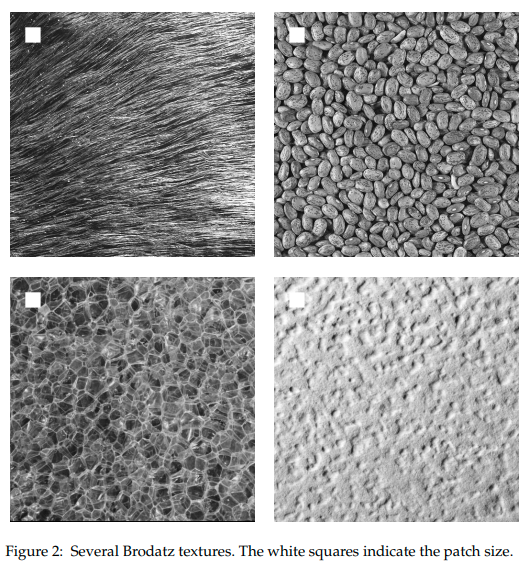
\includegraphics[width=0.4\linewidth]{imagens/brodatz.png}
\end{frame}

%Slide
\begin{frame}
\frametitle{Note 3}
\framesubtitle{Result details}
SMEM\footnote{\begin{scriptsize}Split and Merge EM is a variant of the standard EM where the algo checks after EM convergence if the log-likelihood can be improved by splitting one mixture component in two and merging two other mixture components\end{scriptsize}} and the greedy method are roughly comparable in results given the average conditional entropy\footnote{\begin{scriptsize}It measure quantifies the amount of info. necessary to describe the results of a RV $Y$ given that the value of another RV $X$ is known\end{scriptsize}} measure compared to other methods included K-Means initialized EM GMM. The results were achieved much faster for the greedy method compared to SMEM.
\begin{figure}
    \centering
    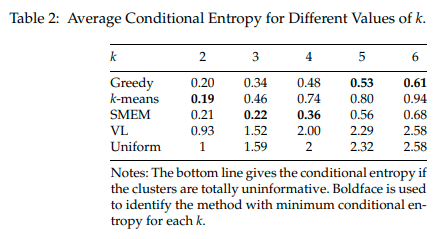
\includegraphics[width=0.4\linewidth]{imagens/results.png}
\end{figure}
\end{frame}

\end{document}